\section*{Задание}
\quad Описать распределения и реализовать программу для построения графиков функции распределения и
функции плотности распределения для следующих распределений:
\begin{itemize}[label=---]
	\item гиперэкспоненциальное распределение;
	\item равномерное распределение.
\end{itemize}

\section*{Равномерное распределение}
\quad Равномерное распределение — распределение случайной величины, принимающей значения, принадлежащие некоторому промежутку конечной длины, характеризующееся тем, что плотность вероятности на этом промежутке всюду постоянна.

Равномерное распределение обозначают $X \sim R(a, b)$, где a, b $\in$ R. 

Функция распределения равномерной непрерывной случайной величины:
\begin{equation}
	F(x) = \begin{cases}
		0 \text{, при } x \geq a\\\\
		\frac{x-a}{b-a} \text{, при } a \leq x \leq b\\\\
		1 \text{, при } x > b
	\end{cases}.
\end{equation}
Плотность распределения равномерной непрерывной случайной величины:
\begin{equation}
	f(x) = \begin{cases}
		\frac{1}{b-a} \text{, при } a \leq x \leq b\\\\
		0 \text{, иначе }
	\end{cases}.
\end{equation}
\clearpage

\section*{Гиперэкспоненциальное распределение}
\quad 

Гиперэкспоненциальное распределение имеет функцию распределения вида:
\begin{equation}
	F_{X}(x) = \begin{cases}
	\sum_{i=1}^n F_{Y_{i}}(y, \lambda_{i}) * p_{i} \text{, при } x \geq 0\\\\
		0 \text{, иначе }
	\end{cases}
\end{equation}

и функцию плотности вида:
\begin{equation}
	f_{X}(x) = \begin{cases}
		\sum_{i=1}^n f_{Y_{i}}(y, \lambda_{i}) * p_{i} \text{, при } x \geq 0\\\\
		0 \text{, иначе }
	\end{cases},
\end{equation}
где:
\begin{itemize}[label=---]
	\item $F_{Y_{i}}(y, \lambda)$ - функция распределения экспоненциальной случайной величины $Y_{i}$ с параметром $\lambda_{i} > 0$, имеющая вид:
	\begin{equation}
		F_{X}(x, \lambda) = \begin{cases}
			1 - e^{-\lambda x} \text{, при } x \geq 0\\\\
			0 \text{, иначе }
		\end{cases};
	\end{equation}
	\item $f_{Y_{i}}(y, \lambda)$ - функция плотности распределения экспоненциальной случайной величины $Y_{i}$ с параметром $\lambda_{i} > 0$, имеющая вид:
	\begin{equation}
		f_{X}(x, \lambda) = \begin{cases}
			\lambda e^{-\lambda x} \text{, при } x \geq 0\\\\
			0 \text{, иначе }
		\end{cases};
	\end{equation}
	
	\item $p_{i}$ -- вероятность того, что случайная величина X будет иметь экспоненциальное распределение с параметром $\lambda_{i}$, $p_{i} > 0$ и $\sum_{i=1}^n p_{i} = 1$.
\end{itemize}

\clearpage

\section*{Результаты работы программы}

\begin{figure}[h]
	\centering
	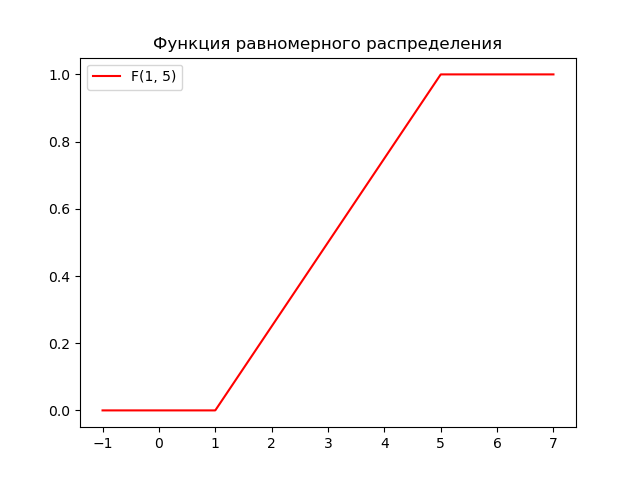
\includegraphics[scale = 0.45]{img/1.png}
	\label{fig:screenshot001}
	\caption{График функции равномерного распределения при a = 1, b = 5}
\end{figure}

\begin{figure}[h]
	\centering
	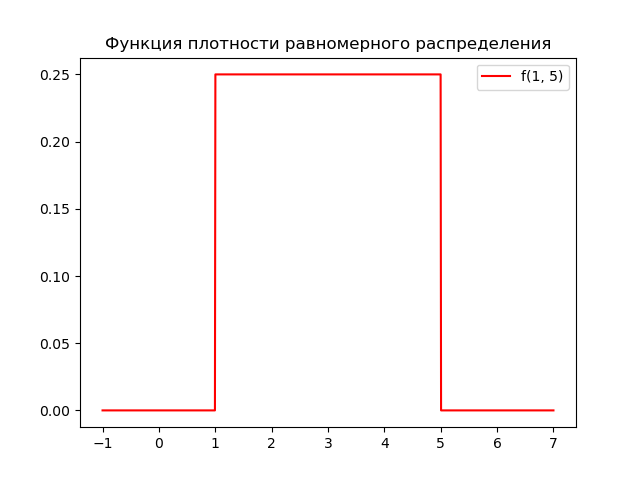
\includegraphics[scale = 0.45]{img/2.png}
	\label{fig:screenshot002}
	\caption{График функции плотности равномерного распределения при a = 1, b = 5}
\end{figure}

\begin{figure}[h]
	\centering
	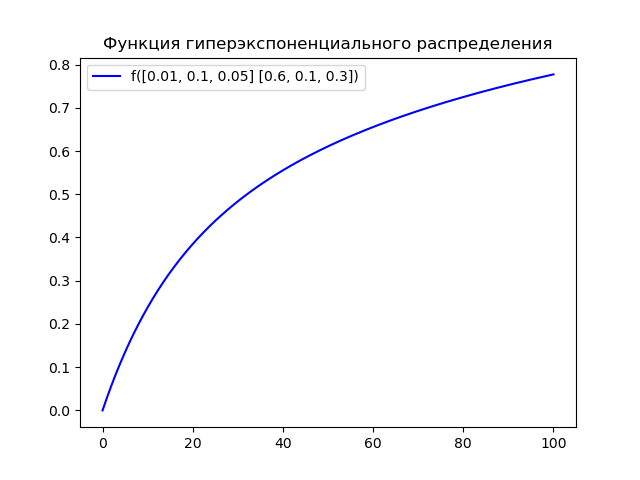
\includegraphics[scale = 0.5]{img/3.png}
	\label{fig:screenshot003}
	\caption{График функции гиперэкспоненциальное распределения при $\lambda$ = [0.01, 0.1, 0.05], p = [0.6, 0.1, 0.3]}
\end{figure}

\begin{figure}[h]
	\centering
	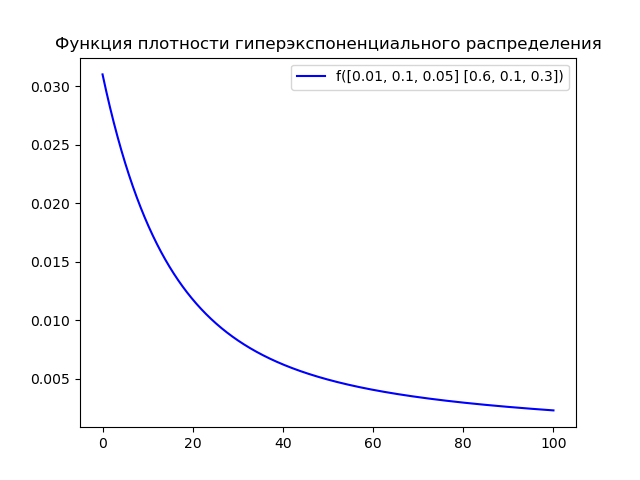
\includegraphics[scale = 0.5]{img/4.png}
	\label{fig:screenshot004}
	\caption{График функции плотности гиперэкспоненциальное распределения при $\lambda$ = [0.01, 0.1, 0.05], p = [0.6, 0.1, 0.3]}
\end{figure}
\end{document}
